\chapter{वर्कशीट की फॉरमेटिंग}

एमएस एक्सेल शीट पर कई प्रकार कि फॉरमेटिंग लागू कि जा सकती हैं। एक्सेल आपकी वर्कशीट को अधिक प्रोफेशनल लुकिंग बनाने के लिए फॉरमेटिंग के अनेक विकल्प प्रदान करता है, जिससे आपके डेटा को प्रभावी ढंग से प्रदर्शित किया जा सके। आप नंम्बर फॉर्मेट का उपयोग करके नंबर को एक निश्चित तरीके से प्रदर्शित कर सकते है, उदाहरण के लिए, वैज्ञानिक फॉर्मेट नंम्बरों के रूप में, डेट्स के रूप मे। आप सेलों का साइज बदलने के लिए, रंगों और बॉर्डर्स को जोड़ने के लिए सेल फॉर्मेटों का उपयोग कर सकते हैं। आप अपने वर्कशीट में टाइपफेस और कैरक्टर्स की स्टाइल को बदलने के लिए फॉन्ट फॉर्मेट का उपयोग कर सकते हैं। एक्सेल 2007 में फॉर्मेटिंग टूल्स तीन स्थान पर उपलब्ध होते हैंः
\begin{enumerate}[topsep=-2ex,parsep=0ex,partopsep=0ex,itemsep=0ex]
\item होम टैब में
\item फॉर्मेट सेल डायलॉग बॉक्स में
\item मिनी टूलबार में जो रेंज या सेल पर दायाँ क्लिक करने पर प्रदर्शित होते हैं
\end{enumerate}

\paragraphTitle{1) होम टैब}
\vskip -10pt

होम टैब, फॉर्मेटिंग आवश्यकताओं के सन्दर्भ में, सामान्यतया प्रयोग किए जाने वाले विकल्पों को आसानी से उपलब्ध कराता है। सबसे अधिक प्रयुक्त फॉरमेटिंग विकल्प होम टैब पर तीन ग्रुप में दिखाइ देते हैंः
\begin{enumerate}[topsep=-1ex,parsep=0ex,partopsep=0ex,itemsep=0.5ex]
\renewcommand{\labelenumi}{\theenumi)}
\item फॉन्ट ग्रुपः फॉन्ट ग्रुप कमांड्स किसी सेल में टेक्स्ट की या सेल की अपीयरेंस को बदलती हैं।
\item एलाइमेंट ग्रुपः एलाइमेंट ग्रुप कमांड्स किसी सेल या सेलों में टेक्स्ट की स्थिति को परिवर्तित करती हैं।
\item नंम्बर ग्रुपः नंम्बर ग्रुप कमांड्स किसी सेल के भीतर नंम्बर और दिनांक का फॉर्मेट बदलती हैं। आप सेल या रेंज को चुनकर इस टूल द्वारा जरूरतों के अनुसार डाटा को बदल सकते हैं, जैसे कि अलाइनमेंट करना, फॉन्ट बदलना या नंम्बर का फॉर्मेट बदलना। ऐसे टूल्स के उचित और बेहतर उपयोग को समझने का एक मात्र तरीका है उनका उपयोग करके उनके प्रभावों को देखना। फॉरमेटिंग परिवर्तन एक पूरी वर्कशीट, वर्कशीट के भीतर सेलों की एक रेंज, अलग-अलग सेलों, और सेल के भीतर के टेक्स्ट के लिए भी लागू किये जा सकते हैं।
\end{enumerate}

\begin{figure}[H]
\centering
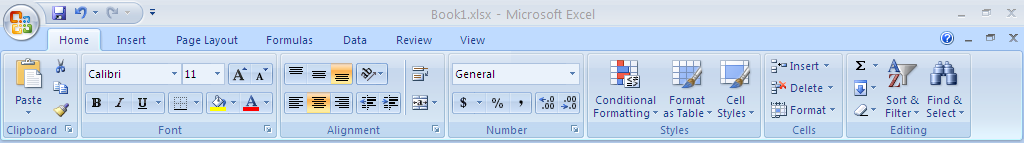
\includegraphics[scale=0.38]{src/images/chapter2/chapter2_fig01.png}
\end{figure}


\paragraphTitle{2) फॉरमेट सेल डायलॉग बॉक्स}

इस डॉयलॉग बॉक्स की मदद से आप किसी भी प्रकार की फॉर्मेटिंग स्टाइल या नंबर फॉर्मेट को लागू कर सकते हैं। फॉर्मेट सेल्स डायलॉग बॉक्स से चयनित फॉर्मेट उन सेल्स पर लागू होता है जो उस समय चयनित होते हैं। फॉर्मेट सेल्स डायलॉग बॉक्स का उपयोग करने के लिए, उस सेल या रेंज का चयन करें जिस पर आपको फॉर्मेटिंग लागू करनी है। आप फॉर्मेट सेल्स डायलॉग बॉक्स लांच करने के लिए Ctrl+1 कमांड का उपयोग, या होम$\to$फॉन्ट, होम$\to$अलाइनमेंट, या होम$\to$नंबर में डायलॉग बॉक्स लॉन्चर पर क्लिक करे या चयनित सेल या रेंज पर राइट-क्लिक करने के बाद शॉर्टकट मेनू से फॉर्मेट सेल का चयन करके कर सकते हैं।
\begin{figure}[H]
\centering
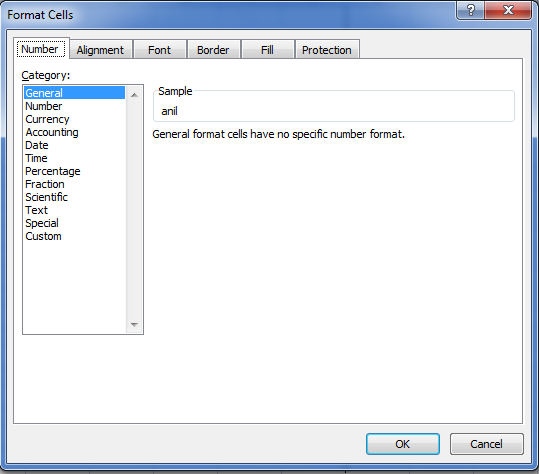
\includegraphics[scale=0.42]{src/images/chapter2/chapter2_fig02.png}
\end{figure}

\paragraphTitle{2) मिनी टूलबार}

जब आप एक सेल या रेंज पर दायाँ क्लिक करते हैं तो शॉर्टकट मेन्यू प्रकट होता है। मिनी टूलबार शॉर्टकट मेन्यू के ऊपर या नीचे प्रकट होता है। मिनी टूलबार में सामान्य फॉर्मेटिंग के लिए कंट्रोल्स होते हैं जैसे कि फॉन्ट, फॉन्ट प्रकार, फॉन्ट साइज़, फॉन्ट घटाना, फॉन्ट बढ़ाना, फॉन्ट कलर, फॉर्मेट पेंटर, बोल्ड, इटैलिक, सेंटर, बॉर्डर, मर्ज एंड सेटंर, डेसिमल बढ़ाना, डेसिमल घटाना और रंग भरना आदि।
\newpage

\begin{figure}[H]
\centering
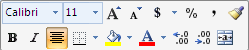
\includegraphics{src/images/chapter2/chapter2_fig03.png}
\end{figure}


\section{फॉर्मेट पेंटर}\label{id-2.1}

फ़ॉर्मेट पेंटर का उपयोग करके आप जल्दी से डाक्युमेंट में, एक चीज की फॉर्मेटिंग को दूसरे में कॉपी कर सकते है। बस उस चीज का चयन करें जिसका लुक आपको पसंद है, फिर फ़ॉर्मेट पेंटर क्लिक करें, और उसके बाद वह चीज जिसे आप वैसा ही लुक देना चाहते हैं, पर क्लिक करें। फ़ॉर्मेट पेंटर आपकी पहली चीज से सभी फोर्मेटिंग को चुन लेता है, चाहे यह कोई आकृति, सेल, पिक्चर बॉर्डर, या टेक्स्ट का भाग हो, और दूसरी चीज पर लागू कर देता है।
\begin{figure}[H]
\centering
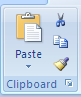
\includegraphics[scale=.87]{src/images/chapter2/chapter2_fig04.png}\qquad
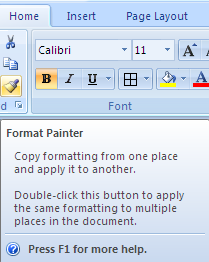
\includegraphics[scale=.87]{src/images/chapter2/chapter2_fig05.png}
\end{figure}

\section{फॉन्ट स्टाइल}\label{id-2.2}

फॉन्ट स्टाइल के चार प्रकार होते हैंः रेगुलर, बोल्ड, इटैलिक और बोल्ड इटैलिक। आप वर्कशीट मे चयनित सेलों या रेंज की फॉन्ट स्टाइल परिवर्तित कर सकते हैं।
\begin{figure}[H]
\centering
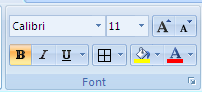
\includegraphics[scale=.8]{src/images/chapter2/chapter2_fig06.png}
\end{figure}

\section{फॉन्ट साइज}\label{id-2.3}

आप फॉन्ट ग्रुप में होम टैब में से उपयुक्त फॉन्ट साइज का चयन करके वर्कशीट की चयनित सेलों या रेंज की फॉन्ट साइज को परिवर्तित कर सकते हैं।
\begin{figure}[H]
\centering
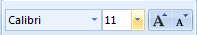
\includegraphics[scale=.8]{src/images/chapter2/chapter2_fig07.png}
\end{figure}

\section{सेल पर बॉर्डर और कलर लागू करना}\label{id-2.4}

जब आप किसी रिक्त वर्कशीट पर देखते हैं तो वहाँ पर कुछ पतली लाइनें होती है जो कि संकेत देती है कि सेल कहॉ हैं, इन लाइनों के बिना शीट में एक विशेष सेल को पहचानना कठिन होता है। लेकिन ये ग्रिड लाइनें केवल ऑक्सीलिरी (सहायक) लाइन्स होती हैं, ये तब तक प्रिन्ट मे नहीं आती हैं जब तक आप विशेष रूप से इसके लिये अनुरोध न करें। आप चयनित सेल (सेलों) पर कोई बॉर्डर और कलर लागू करने के लिये निम्नलिखित चरणों का उपयोग करेः
\begin{descriptionSimple}{चरण 7:}
\item[चरण 1] \textbf{होम} टैब पर, \textbf{सेल} ग्रुप में, \textbf{फॉर्मेट} क्लिक करें
\item[चरण 2] \textbf{फॉर्मेट सेल} डायलॉग बॉक्स प्रदर्शित करने के लिए, \textbf{प्रोटेक्शन} के अंतर्गत, \textbf{फॉर्मेट सेल} क्लिक करें
\item[चरण 3] \textbf{बॉर्डर} टैब का चयन करें
\item[चरण 4] बॉर्डर का लोकेशन स्पेसिफाइ (चिन्हित) करने के लिए, प्रीसेट्स एरिया में \textbf{नन, आउटलाइन,} या \textbf{इनसाइड} विकल्प चुने
\item[चरण 5] बॉर्डर के लिए निम्न में से किसी भी विकल्प को चुनेंः
  \begin{itemize}
    \item बॉर्डर एरिया में, इसकी बॉर्डर को टॉगल करने के लिए किसी भी बटंन पर क्लिक करें
    \item स्टाइल एरिया में बॉर्डर लाइन स्टाइल चुनें
    \item यदि आवश्यक हो तो कलर पैलेट से, बॉर्डर के लिए रंग का चयन करें
  \end{itemize}
\item[चरण 6] \textbf{पैटर्न} टैब का चयन करें, और उसके बाद निम्न विकल्पों में से कोई भी चुनेंः
  \begin{itemize}
    \item कलर पेलेट से सेलेक्शन के बैकग्राउंड के लिए रंग का चयन करें
    \item यदि आवश्यक हो, पैटर्न पैलेट से सेलेक्शन के बैकग्राउंड के लिए पैटर्न का चयन करें
  \end{itemize}
\item[चरण 7] बॉर्डर और कलर लागू करने के लिए ओके चुनें होम टैब में फॉन्ट ग्रुप के बॉर्डर मेनू के विकल्पो का उपयोग करके भी चयनित सेल (सेलों) पर आप बॉर्डर और कलर लागू कर सकते हैं।
\end{descriptionSimple}
\bigskip

\begin{figure}[H]
\centering
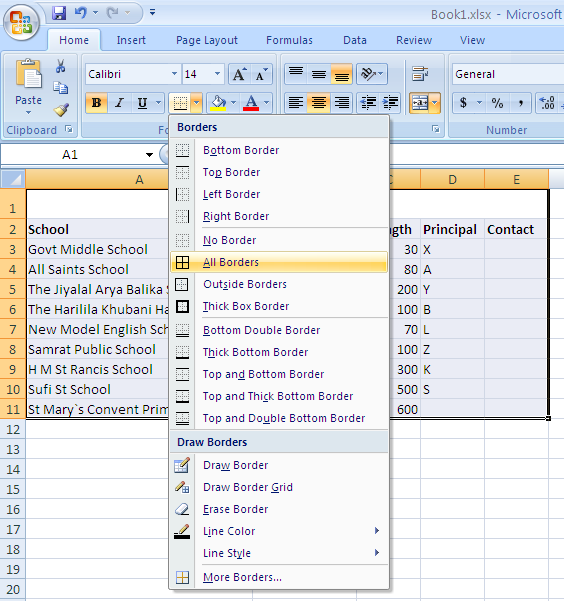
\includegraphics[scale=.7]{src/images/chapter2/chapter2_fig08.png}
\end{figure}
\newpage

\begin{figure}[H]
\centering
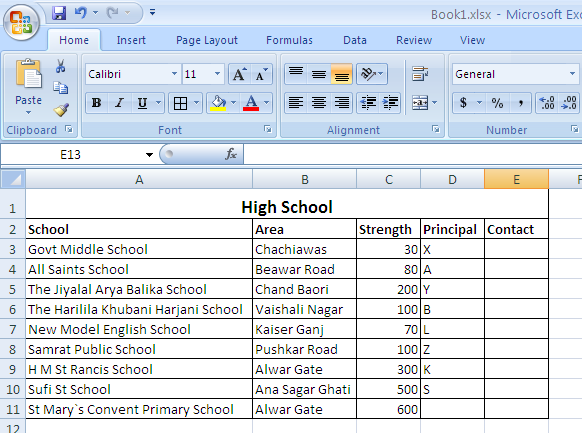
\includegraphics[scale=.6]{src/images/chapter2/chapter2_fig09.png}
\end{figure}

\section{रो और कॉलम की चौड़ाई बदलना}\label{id-2.5}


\paragraphTitle{रो की ऊंचाई सेट करना}
\vskip -10pt

एक या एक से अधिक रो की विशिष्ट ऊंचाई (हाइट) सेट करने के लिए, उस या उन रो का चयन करें जिसे आप बदलना चाहते हैं और निम्न चरणों का उपयोग करेः
\begin{descriptionSimple}{चरण 3:}
\item[चरण 1] \textbf{होम} टैब पर, \textbf{सेल} ग्रुप में, \textbf{फॉर्मेट} क्लिक करें
\item[चरण 2] \textbf{सेल साइज} के तहत, \textbf{रो हाइट} क्लिक करें
\item[चरण 3] \textbf{रो हाइट} डायलॉग बॉक्स में, वह मान लिखें जो आप चाहते हैं
\end{descriptionSimple}
आप \textbf{होम} टैब के \textbf{फॉर्मेट} ग्रुप मे, \textbf{सेल साइज} के अंतर्गत, \textbf{ऑटोफिट रो हाइट} का उपयोग करके, कन्टेंन्स को फिट करने के लिए रो हाइट को सेट कर सकते हैं।

\paragraphTitle{कॉलम की चौड़ाई सेट करना}
\vskip -10pt

कॉलम (कॉलमों) के लिए विशिष्ट चौड़ाई (विड्थ) सेट करने के लिए, कॉलम या कॉलमों का चयन करें जिसे आप बदलना चाहते हैं और निम्न चरणों का उपयोग करेंः

\newpage

\begin{descriptionSimple}{चरण 3:}
\item[चरण 1] \textbf{होम} टैब पर, \textbf{सेल} ग्रुप में, \textbf{फॉर्मेट} क्लिक करें
\item[चरण 2] \textbf{सेल साइज} के तहत, \textbf{कॉलम विड्थ } क्लिक करें
\item[चरण 3] \textbf{कॉलम विड्थ } डायलॉग बॉक्स में, वह मान लिखें जो आप चाहते हैं
\end{descriptionSimple}
आप \textbf{होम} टैब के \textbf{फॉर्मेट} ग्रुप मे, \textbf{सेल साइज} के अंतर्गत, \textbf{ऑटोफिट कॉलम विड्थ } का उपयोग करके, कन्टेंन्स को फिट करने के लिए कॉलम (कॉलमो) कि विड्थ को सेट कर सकते हैं।
\begin{figure}[H]
\centering
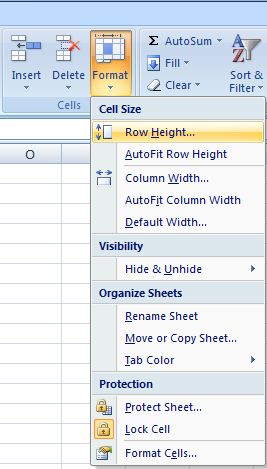
\includegraphics[scale=.75]{src/images/chapter2/chapter2_fig10.png}\qquad
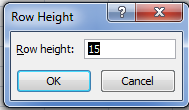
\includegraphics[scale=.75]{src/images/chapter2/chapter2_fig11.png}
\end{figure}

\newpage

\begin{figure}[H]
\centering
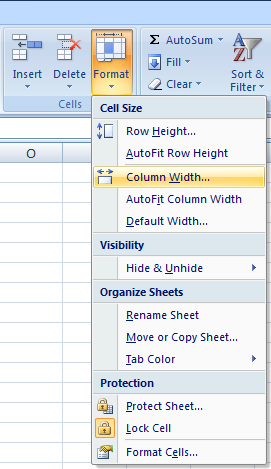
\includegraphics[scale=.75]{src/images/chapter2/chapter2_fig12.png}\qquad
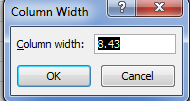
\includegraphics[scale=.75]{src/images/chapter2/chapter2_fig13.png}
\end{figure}

\section{रो और कॉलम की चौड़ाई माउस का उपयोग करके बदलना}\label{id-2.6}

माउस का उपयोग करके, रो की हाइट परिवर्तित करने के लिए, निम्न में से एक का उपयोग करेः
\begin{enumerate}
\renewcommand{\labelenumi}{\theenumi)}
\item एक रो की हाइट बदलने के लिए, रो के शीर्षक के नीचे की सीमा को तब तक ड्रैग करें जब तक रो की ऊंचाई वह न हो जाए जो आप चाहते हैं।
\item एक से अधिक रो की हाइट बदलने के लिए, उन रो का चयन करें जिन्हें आप बदलना चाहते हैं, और उसके बाद किसी भी एक चयनित रो के शीर्षक के नीचे की सीमा ड्रैग करें।

\newpage

\item वर्कशीट पर सभी रो की हाइट बदलने के लिए, \textbf{सेलेक्ट ऑल} बटन क्लिक करें और उसके बाद किसी भी रो शीर्षक के नीचे की सीमा को ड्रैग करें।
\item कन्टेंन्स को फिट करने के लिए, रो की हाइट परिवर्तित करने के लिए चयनित रो के शीर्षक के नीचे की सीमा पर डबल क्लिक करें।
\end{enumerate}

\begin{figure}[H]
\centering
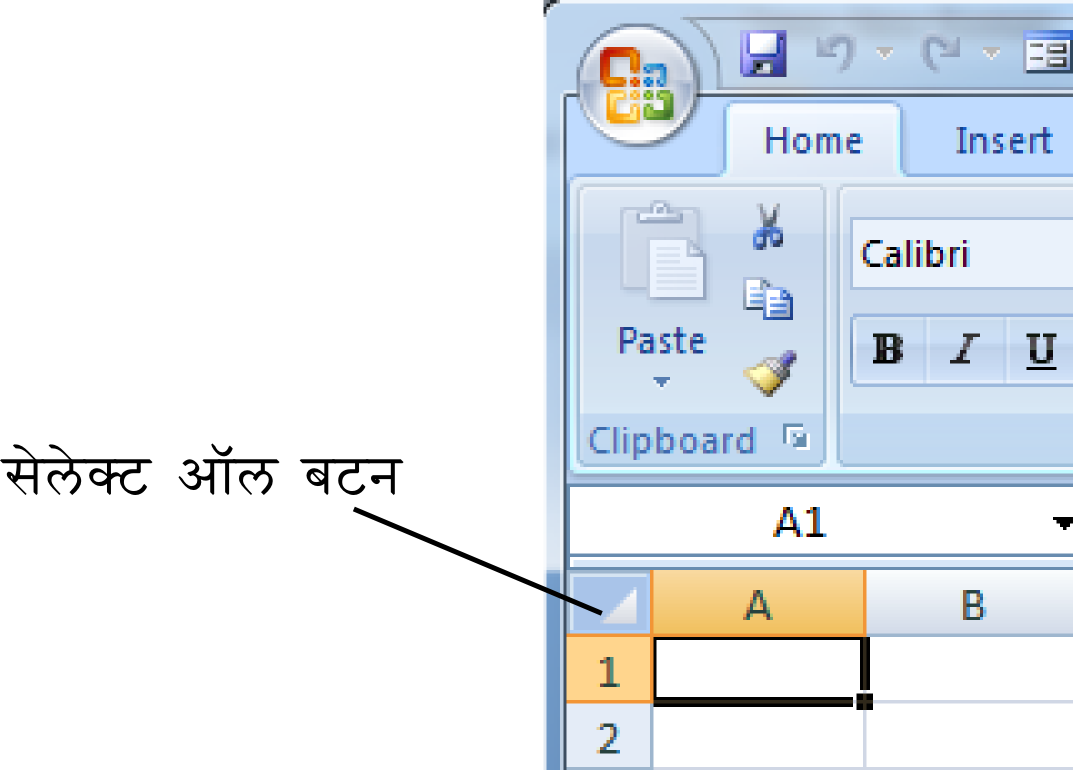
\includegraphics[scale=.75]{src/images/chapter2/chapter2_fig14.png}
\end{figure}
माउस का उपयोग करके, कॉलम की विड्थ परिवर्तित करने के लिए, निम्न में से एक का उपयोग करेः
\begin{enumerate}
\renewcommand{\labelenumi}{\theenumi)}
\item एक कॉलम की विड्थ बदलने के लिए, कॉलम शीर्षक के दाईं ओर की सीमा तब तक खींचें जब तक कॉलम की विड्थ वांछित सीमा तक न पहुंच जाए।
\item एक से अधिक कॉलम की विड्थ बदलने के लिए, उन कॉलमों का चयन करें जिन्हें आप बदलना चाहते हैं, और उसके बाद चयनित कॉलम के शीर्षक के दाईं ओर की सीमा को ड्रैग करें।
\item कन्टेंन्स को फिट करने के लिए कॉलम की विड्थ बदलने हेतु उस/उन कॉलम या कॉलमों का चयन करें जिसे आप बदलना चाहते हैं और उसके बाद चयनित कॉलम के शीर्षक की दाईं सीमा पर डबल क्लिक करें।
\item वर्कशीट के सभी कॉलमों की विड्थ बदलने के लिए, \textbf{सेलेक्ट ऑल} बटन पर क्लिक करें और उसके बाद किसी भी कॉलम के शीर्षक की सीमा खींचें।
\end{enumerate}

\section{नम्बर फॉर्मेट लागू करना}\label{id-2.7}

एक्सेल, कैसे एक नंम्बर को किसी सेल में प्रदर्शित करेगा, यह उस सेल के फॉर्मेट पर निर्भर करता है। एक्सेल नंम्बरो को पेरसंटेज, करेंसी, डेट्स इत्यादि के रूप में प्रदर्शित करने के लिए कई विकल्प प्रदान करता है। यदि ये अंतर्निहित फॉर्मेटस् आपकी आवश्यकताओं को पूरा नहीं करते, तो आप अपना स्वयं का फॉर्मेट बनाने के लिए किसी अंतर्निहित नंम्बर फॉर्मेट को अनुकूलित (कस्टमाइज) कर सकते हैं। सेल (सेलों) के लिए एक विशिष्ट फॉर्मेट लागू करने के लिए निम्न चरणों का पालन उपयोग करेः
\begin{descriptionSimple}{चरण 4:}
\item[चरण 1] फॉर्मेट करने के लिए इच्छित सेल (सेलों) का चयन करें
\item[चरण 2] राइट-क्लिक करें और फिर पॉपअप मेनू से \textbf{फॉर्मेट सेल} का चयन करें या \textbf{होम} टैब के \textbf{नंम्बर} ग्रुप पर जाएँ
\item[चरण 3] \textbf{फॉर्मेट सेल} डायलॉग बॉक्स से \textbf{नंम्बर} टैब का चयन करें
\item[चरण 4] एक उपयुक्त श्रेणी और अन्य विकल्प चुनें, और फिर ओके क्लिक करें
\end{descriptionSimple}

अगर सेल में टेक्स्ट और नम्बर हैं और उसमें कोई भी विशेष नंबर फॉर्मेट नहीं है तो जनरल चुनें। इससे यदि आप नंबर कैटेगरी को चुनते है तो आप नम्बर को पूर्णांक (इन्टीजर्स), दशमलव (डेसिमल्स) अंक, जिसमें दशमलव के बाद आने वाली संख्या दर्शाने का प्रावधान होता है, इत्यादि में दर्शा सकते हैं। उदाहरण के लिए, यदि आप दशमलव बिंदु के पश्चात सिर्फ तीन अंक ही दिखाना चाहते हो, तो नंबर कैटेगरी पर जाकर डेसीमल प्लेस के लिये तीन को चुनें।
\begin{figure}[H]
\centering
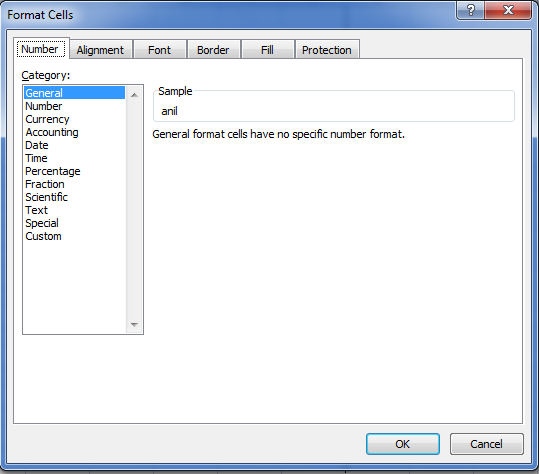
\includegraphics[scale=.7]{src/images/chapter2/chapter2_fig15.png}
\end{figure}

\section{कस्टम नम्बर फॉर्मेट बनाना}\label{id-2.8}

यदि अंतर्निहित नम्बर फॉर्मेट आपकी आवश्यकताओं को पूरा नहीं करता, तो आप एक मौजूदा नम्बर फॉर्मेट पर आधारित, एक नया नम्बर फॉर्मेट बना सकते है और इसे कस्टम नम्बर फॉर्मेटो की सूची मे जोड़ सकते हैं। उदाहरण के लिए, आप ग्राहक जानकारी के लिये स्प्रेडशीट बना रहे हैं, तो आप एक टेलीफोन नंबर के लिए नम्बर फॉर्मेट बना सकते हैं। आप किसी सेल में उन्हें एक टेलीफोन नंबर के रूप में फॉर्मेट करने के लिए, नम्बरों की एक स्ट्रिंग के लिए कस्टम नम्बर फॉर्मेट लागू कर सकते हैं। कस्टम नम्बर फॉर्मेट केवल एक नम्बर को प्रदर्शित करने के तरीके को प्रभावित करते हैं और नम्बर के अंतर्निहित मूल्य (वैल्यु) को प्रभावित नहीं करते। कस्टम नम्बर फॉर्मेट, सक्रिय (एक्टिव) वर्कबुक में ही संग्रहीत किए जाते हैं और खोले जाने वाली नई वर्कबुको के लिए उपलब्ध नहीं होते हैं।
\begin{descriptionSimple}{चरण 6:}
\item[चरण 1] राइट-क्लिक करें और फिर पॉपअप मेनू से \textbf{फॉर्मेट सेलस्} का चयन करें या \textbf{होम} टैब की \textbf{नंम्बर} ग्रुप पर जाएँ
\item[चरण 2] \textbf{फॉर्मेट सेल} डायलॉग बॉक्स से \textbf{नंम्बर} टैब का चयन करें
\item[चरण 3] \textbf{कस्टम} श्रेणी चुनें
\item[चरण 4] \textbf{टाइप} सूची में, अंतर्निहित फॉर्मेट चुनें, जो कि सबसे ज्यादा वैसा दिखता हो जैसा कि आप बनाना चाहते हैं
\item[चरण 5] \textbf{टाइप} बॉक्स में, इच्छित फॉर्मेट बनाने के लिए नम्बर फॉर्मेट कोड को संशोधित करें
\item[चरण 6] जब आप समाप्त कर लें, ओके क्लिक करें
\end{descriptionSimple}
\begin{figure}[H]
\centering
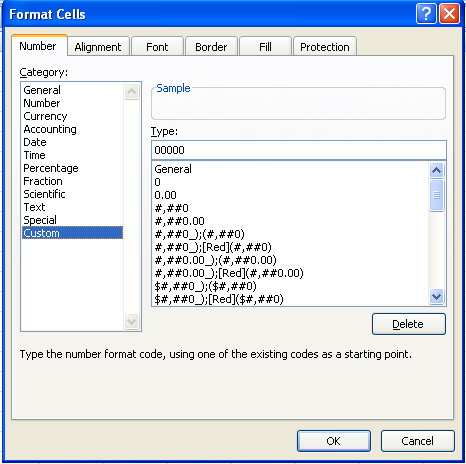
\includegraphics[scale=.58]{src/images/chapter2/chapter2_fig16.png}
\end{figure}

\section{सेल कंटेंट्स को अलाइन करना}\label{id-2.9}

एक्सेल मे \textbf{सेल एलाइमेंट} से अभिप्राय है, कैसे आपका टेक्स्ट या नंम्बर सेल में पोजीशन होंगे। एक्सेल आपको, टेक्स्ट को ऊपर, नीचे, और सेल के बीच में, साथ ही साथ जस्टीफाइ करने के लिए विकल्प और टेक्स्ट को अनुलंब रूप से समायोजित करने के लिए विकल्प प्रदान करता है।

\begin{descriptionSimple}{चरण 4:}
\item[चरण 1] फॉर्मेट करने के लिए इच्छित सेल (सेलों) का चयन करें
\item[चरण 2] राइट-क्लिक करें और फिर पॉपअप मेनू से \textbf{फॉर्मेट सेल} का चयन करें या \textbf{होम} टैब के \textbf{एलाइमेंट} ग्रुप मे जांए
\item[चरण 3] \textbf{फॉर्मेट सेल} डायलॉग बॉक्स से \textbf{एलाइमेंट} टैब का चयन करें
\item[चरण 4] उपयुक्त विकल्प का चयन करें, फिर ओके क्लिक करें
\end{descriptionSimple}

\begin{figure}[H]
\centering
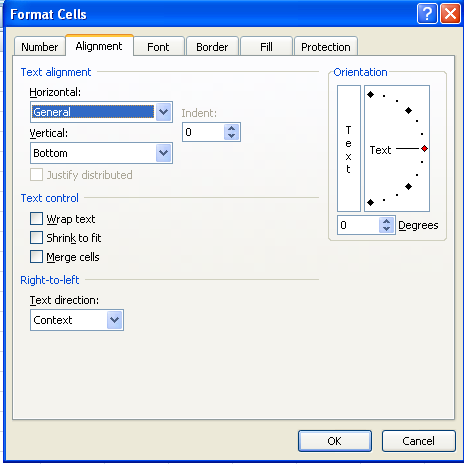
\includegraphics[scale=.62]{src/images/chapter2/chapter2_fig17.png}
\end{figure}


\section{सेल स्टाइल}\label{id-2.10}

एक्सेल 2007 में पूर्वपरिभाषित स्टाइलों का चयन करके आप वर्कशीट को जल्दी से फॉर्मेट कर सकते हैं। एक चरण में कई फॉर्मेटों को लागू करने के लिए, और यह सुनिश्चित करने के लिये कि सेलों की फॉरमेटिंग एकरूप है करने के लिए, आप सेल स्टाइल का उपयोग कर सकते हैं। कोई सेल स्टाइल फॉर्मेटिंग विशेषताओं, जैसे फॉन्ट और फॉन्ट साइजों, नम्बर फॉर्मेटों, सेल बॉर्डर्स, और सेल शैडिंग (छायांकन), का एक निर्धारित सेट है। किसी को विशिष्ट सेलों में परिवर्तन करने से रोकने के लिए, आप भी सेलों को लॉक (अवरोधित) करने वाली सेल स्टाइल का उपयोग कर सकते हैं। एक्सेल मे कई अंतर्निहित सेल स्टाइल होती हैं जिन्हे आप रूपांतरित या संशोधित कर सकते है। एक सेल स्टाइल को संशोधित या सेल स्टाइल को डुप्लिकेट करके भी, आप अपने स्वयं का कस्टम सेल स्टाइल बना सकते हैं। स्टाइल आपकी वर्कशीटों को व्यावसायिक रूप देने में सहायता करती हैं। एक्सेल में सभी स्टाइल, सेल के स्टाइल हैं। हालांकि, परिभाषित स्टाइल को संपूर्ण वर्कशीट पर लागू किया जा सकता है। सेल स्टाइल में कोई भी फॉर्मेटिंग शामिल हो सकती है जिसे उपलब्ध विकल्पों का उपयोग करके सेल में लागू किया जा सकता है।

\begin{descriptionSimple}{चरण 4:}
\item[चरण 1] एक स्टाइल लागू करने के लिए सेल (सेलों) का चयन करें
\item[चरण 2] \textbf{होम} टैब के \textbf{स्टाइल} ग्रुप पर जाए
\item[चरण 3] \textbf{सेल स्टाइल} क्लिक करें
\item[चरण 4] इच्छित \textbf{सेल स्टाइल} क्लिक करें<
\end{descriptionSimple}

आप अलग-अलग सेल स्टाइल ट्राइ कर सकते है, और प्रभाव देख सकते है।

\begin{figure}[H]
\centering
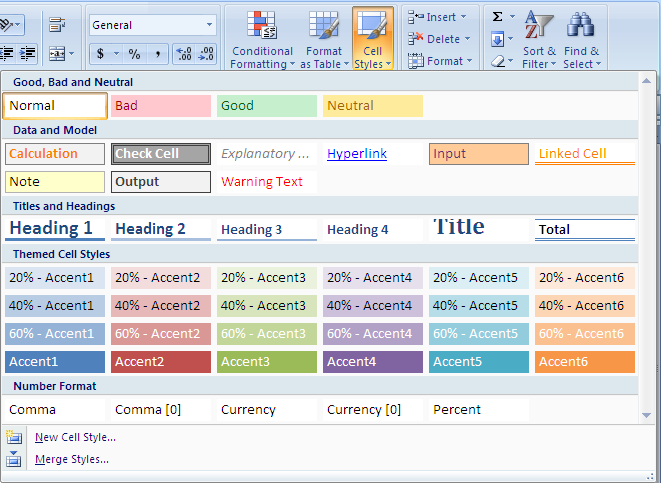
\includegraphics[scale=.59]{src/images/chapter2/chapter2_fig18.png}
\end{figure}

\newpage

\section{अपनी सेल स्टाइल्स बनाना}\label{id-sec2.11}

एक्सेल में अंतर्निहित स्टाइल हर तरह की फॉरमेटिंग की जरूरत को कवर (पूरा) नहीं कर सकते हैं। आप आसानी से अपनी जरूरत के अनुसार अपनी सेल स्टाइल बना सकते हैं। अपनी सेल स्टाइल बनाने के लिए चरणों का पालन करेंः
\begin{descriptionSimple}{चरण 7:}
\item[चरण 1] \textbf{होम} टैब के \textbf{स्टाइल्स} ग्रुप पर जाए
\item[चरण 2] \textbf{सेल स्टाइल्स} क्लिक करें
\item[चरण 3] \textbf{न्यु सेल स्टाइल} क्लिक करें
\item[चरण 4] \textbf{स्टाइल नेम} बॉक्स में, नई स्टाइल के लिए एक नाम टाइप करें
\item[चरण 5] \textbf{फॉर्मेट} क्लिक करें, \textbf{फॉर्मेट सेल} डायलॉग बॉक्स दिखाई देगा
\item[चरण 6] इच्छित फॉरमेटिंग के लिये उपयुक्त विकल्पो को सेट करें, और फिर ओके क्लिक करें
\item[चरण 7] \textbf{स्टाइल} डायलॉग बॉक्स में, \textbf{स्टाइल इन्कलूड्स} के अंतर्गत, स्टाइल फॉरमेटिंग चुनने के लिए, उपयुक्त बोक्सेज को चेक करें और फिर ओके क्लिक करें
\end{descriptionSimple}
कोई मौजूदा स्टाइल पर आधारित एक कस्टम सेल स्टाइल बनाएँः
\begin{descriptionSimple}{चरण 6:}
\item[चरण 1] \textbf{होम} टैब पर, \textbf{फॉर्मेट} के अंतर्गत, किसी भी स्टाइल पर इंगित करें, और उसके बाद क्लिक करें
\item[चरण 2] कण्ट्रोल को दबाये रखे, जो स्टाइल आप चाहते हैं उस पर क्लिक करें और फिर \textbf{डुप्लिकेट} क्लिक करें
\item[चरण 3] \textbf{स्टाइल नेम} बॉक्स में, नई स्टाइल के लिए एक नाम टाइप करें
\item[चरण 4] \textbf{फॉर्मेट} क्लिक करें, \textbf{फॉर्मेट सेल} डायलॉग बॉक्स दिखाई देगा
\item[चरण 5] इच्छित फॉरमेटिंग के लिये उपयुक्त विकल्पो को सेट करें, और फिर ओके क्लिक करें
\item[चरण 6] \textbf{स्टाइल} डायलॉग बॉक्स में, \textbf{स्टाइल इन्कलूड्स} के अंतर्गत, स्टाइल फॉरमेटिंग चुनने के लिए, उपयुक्त बोक्सेज को चेक करें और फिर ओके क्लिक करें
\end{descriptionSimple}

\begin{figure}[H]
\centering
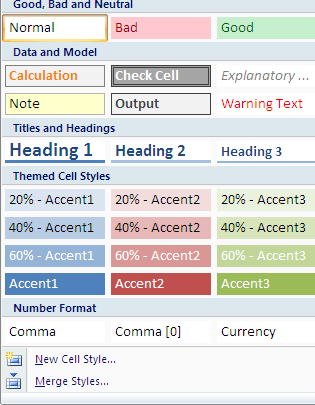
\includegraphics[scale=.5]{src/images/chapter2/chapter2_fig19.png}
\end{figure}

\begin{figure}[H]
\centering
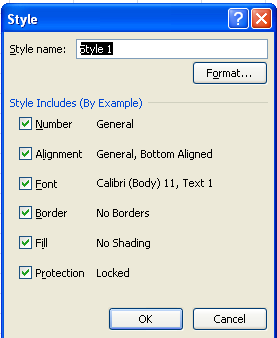
\includegraphics[scale=.55]{src/images/chapter2/chapter2_fig20.png}
\end{figure}

\section{कंडीशनल फॉरमेटिंग}\label{id-2.12}

कंडीशनल फॉरमेटिंग बहुत अधिक लचीली (फ्लेक्सिबल) होती है, यह केवल एक सेल या सेलों की रेंज, जो निश्चित मापदंड या शर्तों (कंडीशन) से मेल खाती हैं, को फॉर्मेट करने देता हैं। उदाहरण के लिए, आप किसी सेल का मान 100 से कम होने पर ही वह सेल बोल्ड प्रकट हो, ऐसा कर सकते है।

जब सेल का मान फॉर्मेट शर्त को पूरा करता है, तब आपके द्वारा चयनित फॉर्मेट सेल के लिए लागू होता है। यदि सेल का मान फॉर्मेट शर्त को पूरी नहीं करता, तो उस सेल की डिफॉल्ट फॉरमेटिंग का उपयोग किया जाता है। यहाँ डिफॉल्ट फॉरमेटिंग द्वारा मतलब उस फॉरमेटिंग से है जिसे आप सामान्य फॉरमेटिंग टुल्स का उपयोग करके सेट करते हैं।

डिफॉल्ट मान (नो फॉरमेटिंग) के अलावा, एक सेल मे तीन फॉर्मेट कंडीशन, प्रत्येक अपने स्वयं के फॉर्मेट के साथ, हो सकती हैं। यह आपको सेल की वैल्यु के आधार पर विभिन्न स्वरूपों (फॉर्मेट) की अनुमति देता है। उदाहरण के लिए, यदि मूल्य 100 से भी कम था, तो आप टेक्स्ट को लाल रंग में प्रदर्शित कर सकते हैं, लेकिन अगर मूल्य 100 और 200 के बीच है, तब हरे रंग में टेक्स्ट प्रदर्शित कर सकते हैं। मान लीजिए आपके पास एक वस्तु सूची है, जिसमे एकाधिक आइटम्स और उनकी स्टॉक में मात्रा हैं। जब एक आइटम की स्टॉक में मात्रा 100 से नीचे तक पहुँच जाती है, यह आपके लिये पता लगाना महत्वपूर्ण हो सकता है, ताकी आप उस विशेष आइटम की ज्यादा यूनिट खरीद सके। यदि आपको कंडीशन फॉरमेटिंग के बारे में पता नहीे हैं, कॉलम में कोई भी नम्बर 100 के नीचे है यह पता करने के लिये, आप अपने स्क्रीन पर अपनी उंगली की नोक को रखकर उसे नीचे की तरफ देखने के लिए आगे बढ़ाना शुरू हो जायेगे। यह कई रो के साथ एक डाटासेट में एक बहुत प्रभावी तरीका नहीं है। कंडीशन फॉरमेटिंग लागू करने के लिए निम्न चरणों का पालन करेः
\begin{descriptionSimple}{चरण 5:}
\item[चरण 1] कंडीशनल फॉरमेटिंग लागू करने के लिए इच्छित सेल (सेलों) का चयन करें
\item[चरण 2] \textbf{होम} टैब के \textbf{स्टाइल} ग्रुप में \textbf{कंडीशनल फॉरमेटिंग} बटन पर क्लिक करें
\item[चरण 3] ड्रॉप डाउन मेनू पर इच्छित विकल्प को इंगित करने के लिए और यह जो चयनित सेलों पर लागू करने के लिए विकल्पों में से एक का चयन करें, एक कैस्केडिंग मेनू दिखाई देगा
\item[चरण 4] एक अतिरिक्त डायलॉग बॉक्स प्रकट हो सकता है, यह आपके विकल्प का चयन पर निर्भर करता है
\item[चरण 5] यदि ऐसा है, तो आवश्यक विकल्प बना ले, फिर ओके क्लिक करें
\end{descriptionSimple}

कंडीशनल फॉरमेटिंग हटाने के लिए, \textbf{कंडीशनल फॉरमेटिंग} पर क्लिक करें, और \textbf{क्लियर-रुल} का  चयन करें। एक कैस्केडिंग मेनू प्रकट होता है संपूर्ण शीट से या चयनित सेलों से नियम हटाने के लिये क्लियर-रुलस् फ्राम सेलेक्टेड सेल को चुनें।

\begin{figure}[H]
\centering
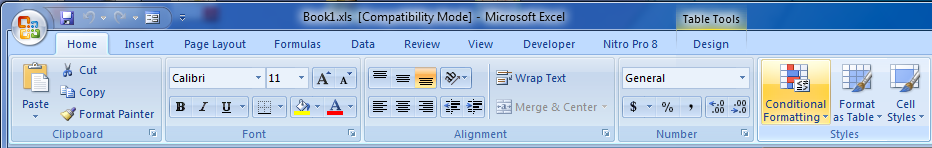
\includegraphics[scale=.42]{src/images/chapter2/chapter2_fig21.png}
\end{figure}

\noindent
\begin{figure}[H]
\centering
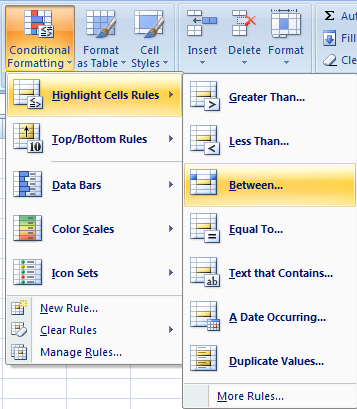
\includegraphics[scale=0.44]{src/images/chapter2/chapter2_fig22.png}\quad
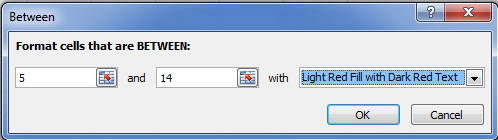
\includegraphics[scale=0.38]{src/images/chapter2/chapter2_fig23.png}
\end{figure}


\section*{महत्वपूर्ण बिंदुः}

\begin{itemize}[topsep=-1ex,parsep=0ex,partopsep=0ex,itemsep=0.4ex]
\item एक्सेल आपकी वर्कशीट को अधिक प्रोफेशनल लुकिंग बनाने के लिए फॉरमेटिंग के अनेक विकल्प प्रदान करता है, जिससे आपके डेटा को प्रभावी ढंग से प्रदर्शित किया जा सके।
\item फ़ॉर्मेट पेंटर का उपयोग करके आप जल्दी से डाक्युमेंट में, एक चीज की फॉर्मेटिंग को दूसरे में कॉपी कर सकते है।
\item फॉन्ट स्टाइल के चार प्रकार होते हैंः रेगुलर, बोल्ड, इटैलिक और बोल्ड इटैलिक।
\item आप होम टैब के फॉर्मेट ग्रुप मे, सेल साइज के अंतर्गत, ऑटोफिट रो हाइट का उपयोग करके, कन्टेंन्स को फिट करने के लिए रो हाइट को सेट कर सकते हैं।
\item कन्टेंन्स को फिट करने के लिए, रो की हाइट परिवर्तित करने के लिए चयनित रो के शीर्षक के नीचे की सीमा पर डबल क्लिक करें।
\item कन्टेंन्स को फिट करने के लिए कॉलम की विड्थ बदलने हेतु उस/उन कॉलम या कॉलमों का चयन करें जिसे आप बदलना चाहते हैं और उसके बाद चयनित कॉलम के शीर्षक की दाईं सीमा पर डबल क्लिक करें।
\item यदि अंतर्निहित नंम्बर फॉर्मेट आपकी आवश्यकताओं को पूरा नहीं करता, तो आप एक कस्टम नंम्बर फॉर्मेट बना़ सकते हैं।
\item एक्सेल मे सेल एलाइमेंट से अभिप्राय है, कैसे आपका टेक्स्ट या नंम्बर सेल में पोजीशन होंगे।
\item एक चरण में कई फॉर्मेटों को लागू करने के लिए, और यह सुनिश्चित करने के लिये कि सेलों की फॉरमेटिंग एकरूप है करने के लिए, आप सेल स्टाइल का उपयोग कर सकते हैं।
\end{itemize}
\section*{अभ्यासार्थ प्रश्न}

\def\paragraphTitle#1{\medbreak\noindent{\bfseries \color{red}{#1}}}
\paragraphTitle{वस्तुनिष्ठ प्रश्नः}
\begin{descriptionSimple}{प्रश्न 1.}
\item[\textbf{प्रश्न 1}] फॉर्मेट पेंटर का उपयोग है

  \begin{tabular}{l@{$\;\;\;$}p{10cm}}
	\textbf{अ.} & अपनी स्लाइड पर सुंदर चित्र पेंट करने के लिए\\
	\textbf{ब.}  & एक ऑब्जेक्ट या टेक्स्ट के भाग से फॉरमेटिंग की प्रतिलिपि (कॅापी) बनाएँ और फिर इसे कहीं और लागू करने के लिए\\
	\textbf{स.}  &अपनी स्लाइड्स की पृष्ठभूमि का रंग बदलने के लिए\\
        \textbf{द.}  & स्लाइड्स की पृष्ठभूमि पर सुंदर चित्र पेंट करने के लिए
  \end{tabular}

\item[\textbf{प्रश्न 2}] किसी एक्सेल शीट पर सक्रिय (एक्टिव) सेल द्वारा दर्शाई जाती है?

  \begin{tabular}{ll}	
	\textbf{अ.} एक डॉटेड बॉर्डर & 
        \textbf{ब.} एक डार्क वाइड बॉर्डर\\
        \textbf{स.} एक ब्लींन्किग बॉर्डर & 
        \textbf{द.} इटैलिक टेक्स्ट द्वारा
  \end{tabular}

\item[\textbf{प्रश्न 3}] एक स्प्रेडशीट में डेटा कैसे संगठित (आर्गनाइज्ड) रहता हैं?

  \begin{tabular}{ll}
    \textbf{अ.} लाइनों और स्पेसेज &
    \textbf{ब.} लेयरस् और प्लेन्स\\
    \textbf{स.} रोज और कॉलमस् &
    \textbf{द.} हाइट और विड्थ
  \end{tabular}

\item[\textbf{प्रश्न 4}] आप किस कमांड् का उपयोग कर, एक्सेल में फॉर्मेट सेल डायलॉग बॉक्स लॉन्च कर सकते हैं?

  \begin{tabular}{llll}
	\textbf{अ.} Ctrl+1 &
        \textbf{ब.} Ctrl+5 &
	\textbf{स.} Ctrl+2 &
	\textbf{द.} Ctrl+3
  \end{tabular}

\item[\textbf{प्रश्न 5}] एक्सेल में ............ प्रकार के फॉन्ट स्टाइल हैं।

  \begin{tabular}{llll}
	\textbf{अ.} 8 &
	\textbf{ब.} 6 &
	\textbf{स.} 4 &
	\textbf{द.} 2
  \end{tabular}

\item[\textbf{प्रश्न 6}] सेल फॉर्मेट डायलॉग बॉक्स में कौन सा टैब उपलब्ध नहीं है?

  \begin{tabular}{llll}
    \textbf{अ.} नंम्बर &
    \textbf{ब.} फॉन्ट &
    \textbf{स.} फील &
    \textbf{द.} मारजिंस
  \end{tabular}
\end{descriptionSimple}

\paragraphTitle{अतिलघूत्तरात्मक प्रश्नः}
\begin{descriptionSimple}{\textbf{प्रश्न 1.}}
\item[\textbf{प्रश्न 1}] फॉर्मेट पेंटर का क्या उपयोग है?
\item[\textbf{प्रश्न 2}] क्या कस्टम नंम्बर फॉर्मेट, नम्बर के अंतर्निहित मूल्य (वैल्यू) को प्रभावित करता है?
\item[\textbf{प्रश्न 3}] एक्सेल के फॉन्ट स्टाइलस् का नाम लिखें।
\item[\textbf{प्रश्न 4}] सेल स्टाइल क्या है?
\item[\textbf{प्रश्न 5}] सेल एलाइमेंट क्या है?
\end{descriptionSimple}

\paragraphTitle{लघूत्तरात्मक प्रश्नः}
\begin{descriptionSimple}{\textbf{प्रश्न 1.}}
\item[\textbf{प्रश्न 1}] रो हाइट और कॉलम विड्थ परिवर्तित करने के चरण लिखे?
\item[\textbf{प्रश्न 2}] फॉर्मेट सेल डायलॉग बॉक्स का उपयोग क्या है?
\item[\textbf{प्रश्न 3}] फ्रीज और अनफ्रीज रोज से आप समझते है?
\item[\textbf{प्रश्न 4}] कंडीशनल फॉरमेटिंग क्या है?
\item[\textbf{प्रश्न 5}] एक्सेल में नम्बर फॉर्मेटों की व्याख्या करे।
\end{descriptionSimple}

\paragraphTitle{निबंधात्मक प्रश्नः}
\begin{descriptionSimple}{\textbf{प्रश्न 1.}}
\item[\textbf{प्रश्न 1}] आप एक्सेल में नंम्बर फॉर्मेट कैसे लागू कर सकते हैं?
\item[\textbf{प्रश्न 2}] कस्टम नंम्बर फॉर्मेट क्या है? कस्टम नंम्बर फॉर्मेट बनाने के लिए चरणों को समझाए।
\item[\textbf{प्रश्न 3}] सेल स्टाइल और अपना स्वयं का सेल स्टाइल बनाने के लिए चरणों को समझाए।
\item[\textbf{प्रश्न 4}] आप सेल मे बॉर्डर और कलर कैसे जोड सकते हैं? समझाए।
\item[\textbf{प्रश्न 5}] वर्कशीट फॉरमेटिंग पर संक्षिप्त टिप्पणी लिखें।
\end{descriptionSimple}

\paragraphTitle{उत्तरमाला}

\begin{tabular}{@{}llllll}
\textbf{उत्तर 1:} ब &
\textbf{उत्तर 2:} ब &
\textbf{उत्तर 3:} स &
\textbf{उत्तर 4:} अ &
\textbf{उत्तर 5:} स &
\textbf{उत्तर 6:} द
\end{tabular}

